\documentclass[../stegner_thesis.tex]{subfiles}

\begin{document}

\chapter{Results}%
\label{ch:results}

\section{Context-Free Model}%
\label{sec:res_context_free}

\par The context-free model was trained on both the Das Malwerk and the BIG
2015 datasets.
The purpose of the context-free model was to test that the LDA models were
producing useful features for comparing the different classes.

\par The context-free classifier for the Das Malwerk dataset for various
numbers of LDA topics is shown in \figref{fig:win32_knn_topics}.
While we tested from 5 topics to 95 topics in multiples of 5, we only plotted
a handful of different numbers of topics against each other for visual clarity.
We have also excluded the error bars for the same reason.
\par In \figref{fig:win32_knn_topics}, there is a clear trend of maximal
accuracy at $k=1$.
To compare all of the LDA models at their peak performance, we plotted their
accuracies with $k$ fixed at 1, shown in \figref{fig:win32_knn_k1}.
The 5 topic LDA model is excluded because its performance was significantly
lower than the others, making the differences between the other models harder
to notice.
The maximal performance occurs with 85 LDA topics at $k=1$, with a
classification accuracy of 95.99\%.

% Context-free Das Malwerk results
\begin{figure}[p]
	\centering
	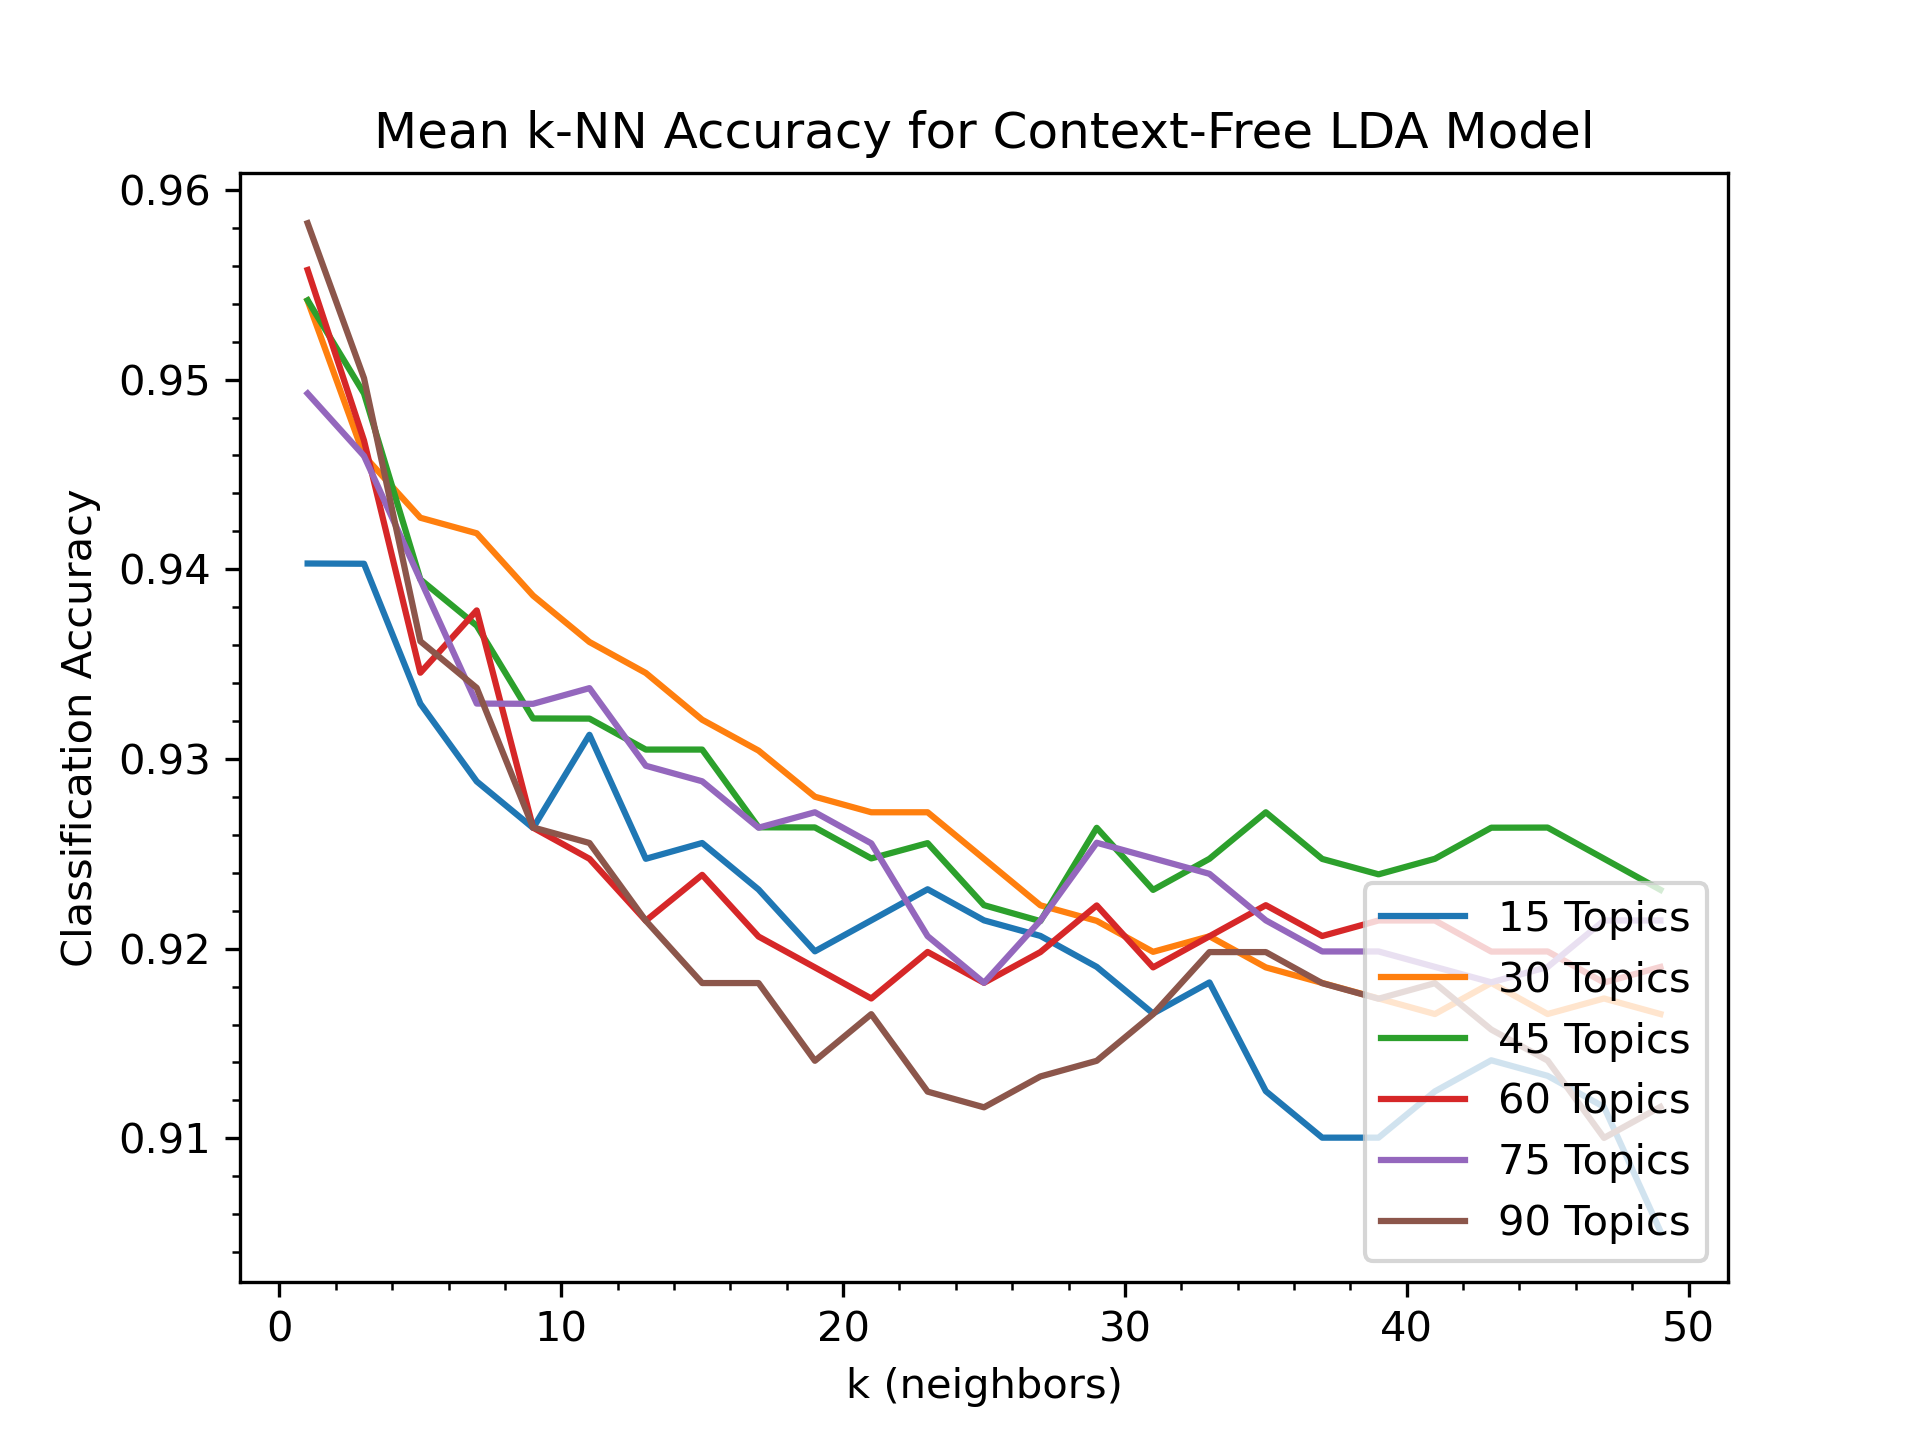
\includegraphics[width=0.75\textwidth]{img/win32/knn_lda.png}
	\caption[Context-free k-NN accuracy vs $k$ for Das Malwerk]{%
		Context-free k-NN accuracy vs $k$ for Das Malwerk.
		For visual clarity, not all numbers of topics are shown and error bars are
		not included.
	}%
	\label{fig:win32_knn_topics}
\end{figure}
\begin{figure}[p]
	\centering
	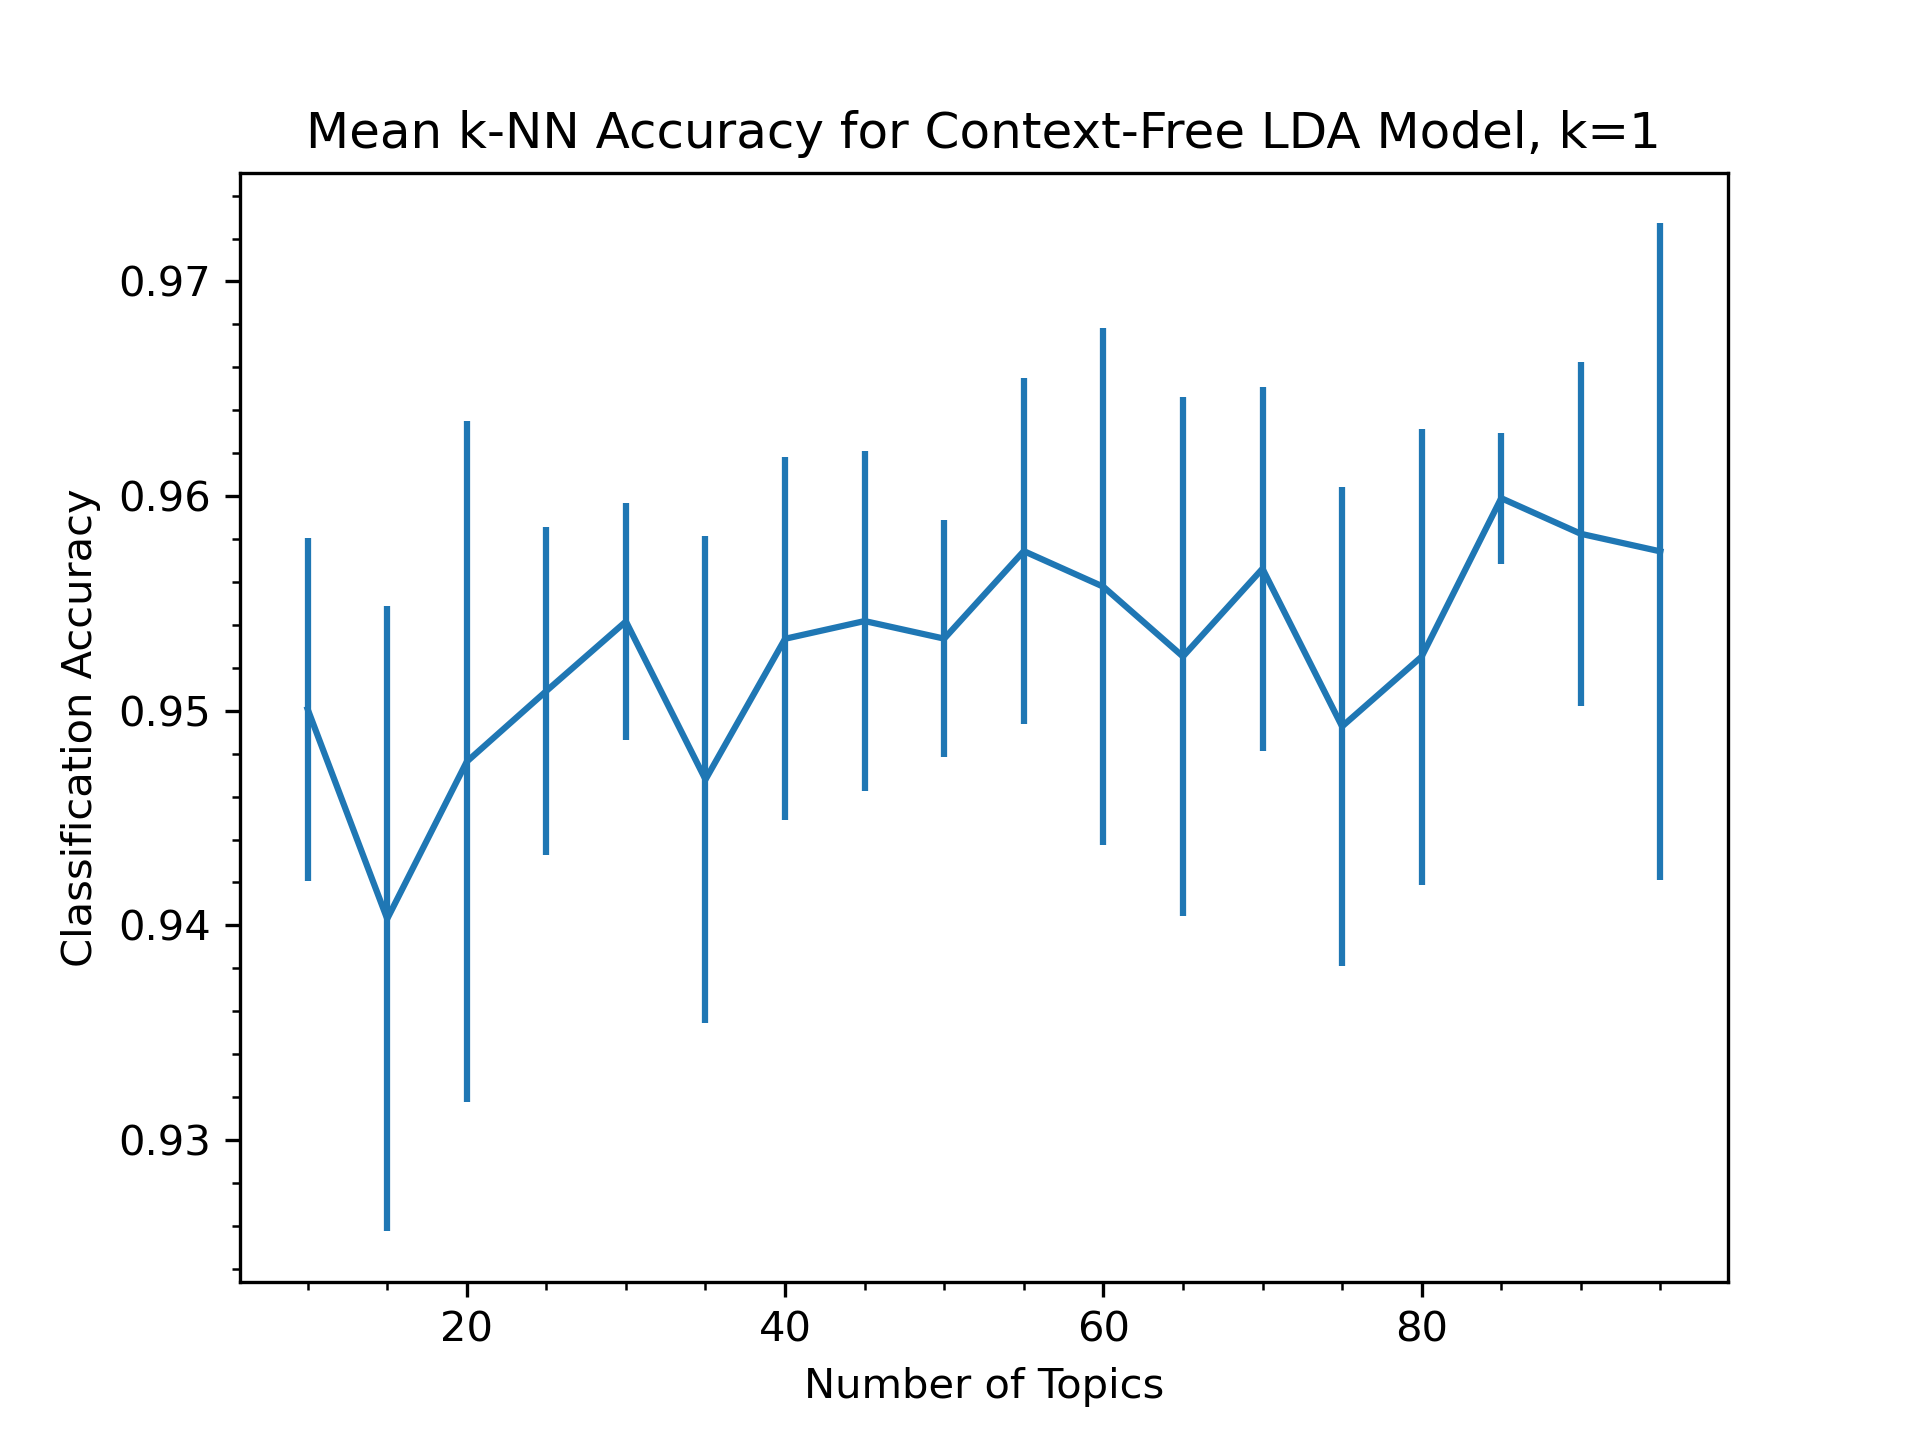
\includegraphics[width=0.75\textwidth]{img/win32/knn_lda_k_01.png}
	\caption[%
		Context-free model k-NN accuracy vs number of topics for Das Malwerk
	]{%
		Context-free model k-NN accuracy vs number of topics for Das Malwerk fixed
		at $k=1$.
		For visual clarity, the 5 topic model is excluded.
	}%
	\label{fig:win32_knn_k1}
\end{figure}

\par The context-free model for the BIG 2015 dataset for various numbers
of LDA topics is shown in \figref{fig:msoft_big_knn_topics}.
However, this time the trend appears where the maximal value for each LDA model
occurs at $k=5$, with the exception of the 15 topic model where $k=1$ is a bit
higher.
We plotted all of the LDA models with $k$ fixed at 5 to compare their best
performances, shown in \figref{fig:msoft_big_knn_k5}.
In this case, the best performing model is with 90 LDA topics at $k=5$, with a
classification accuracy of 97.03\%.

% Context-free BIG 2015 results
\begin{figure}[p]
	\centering
	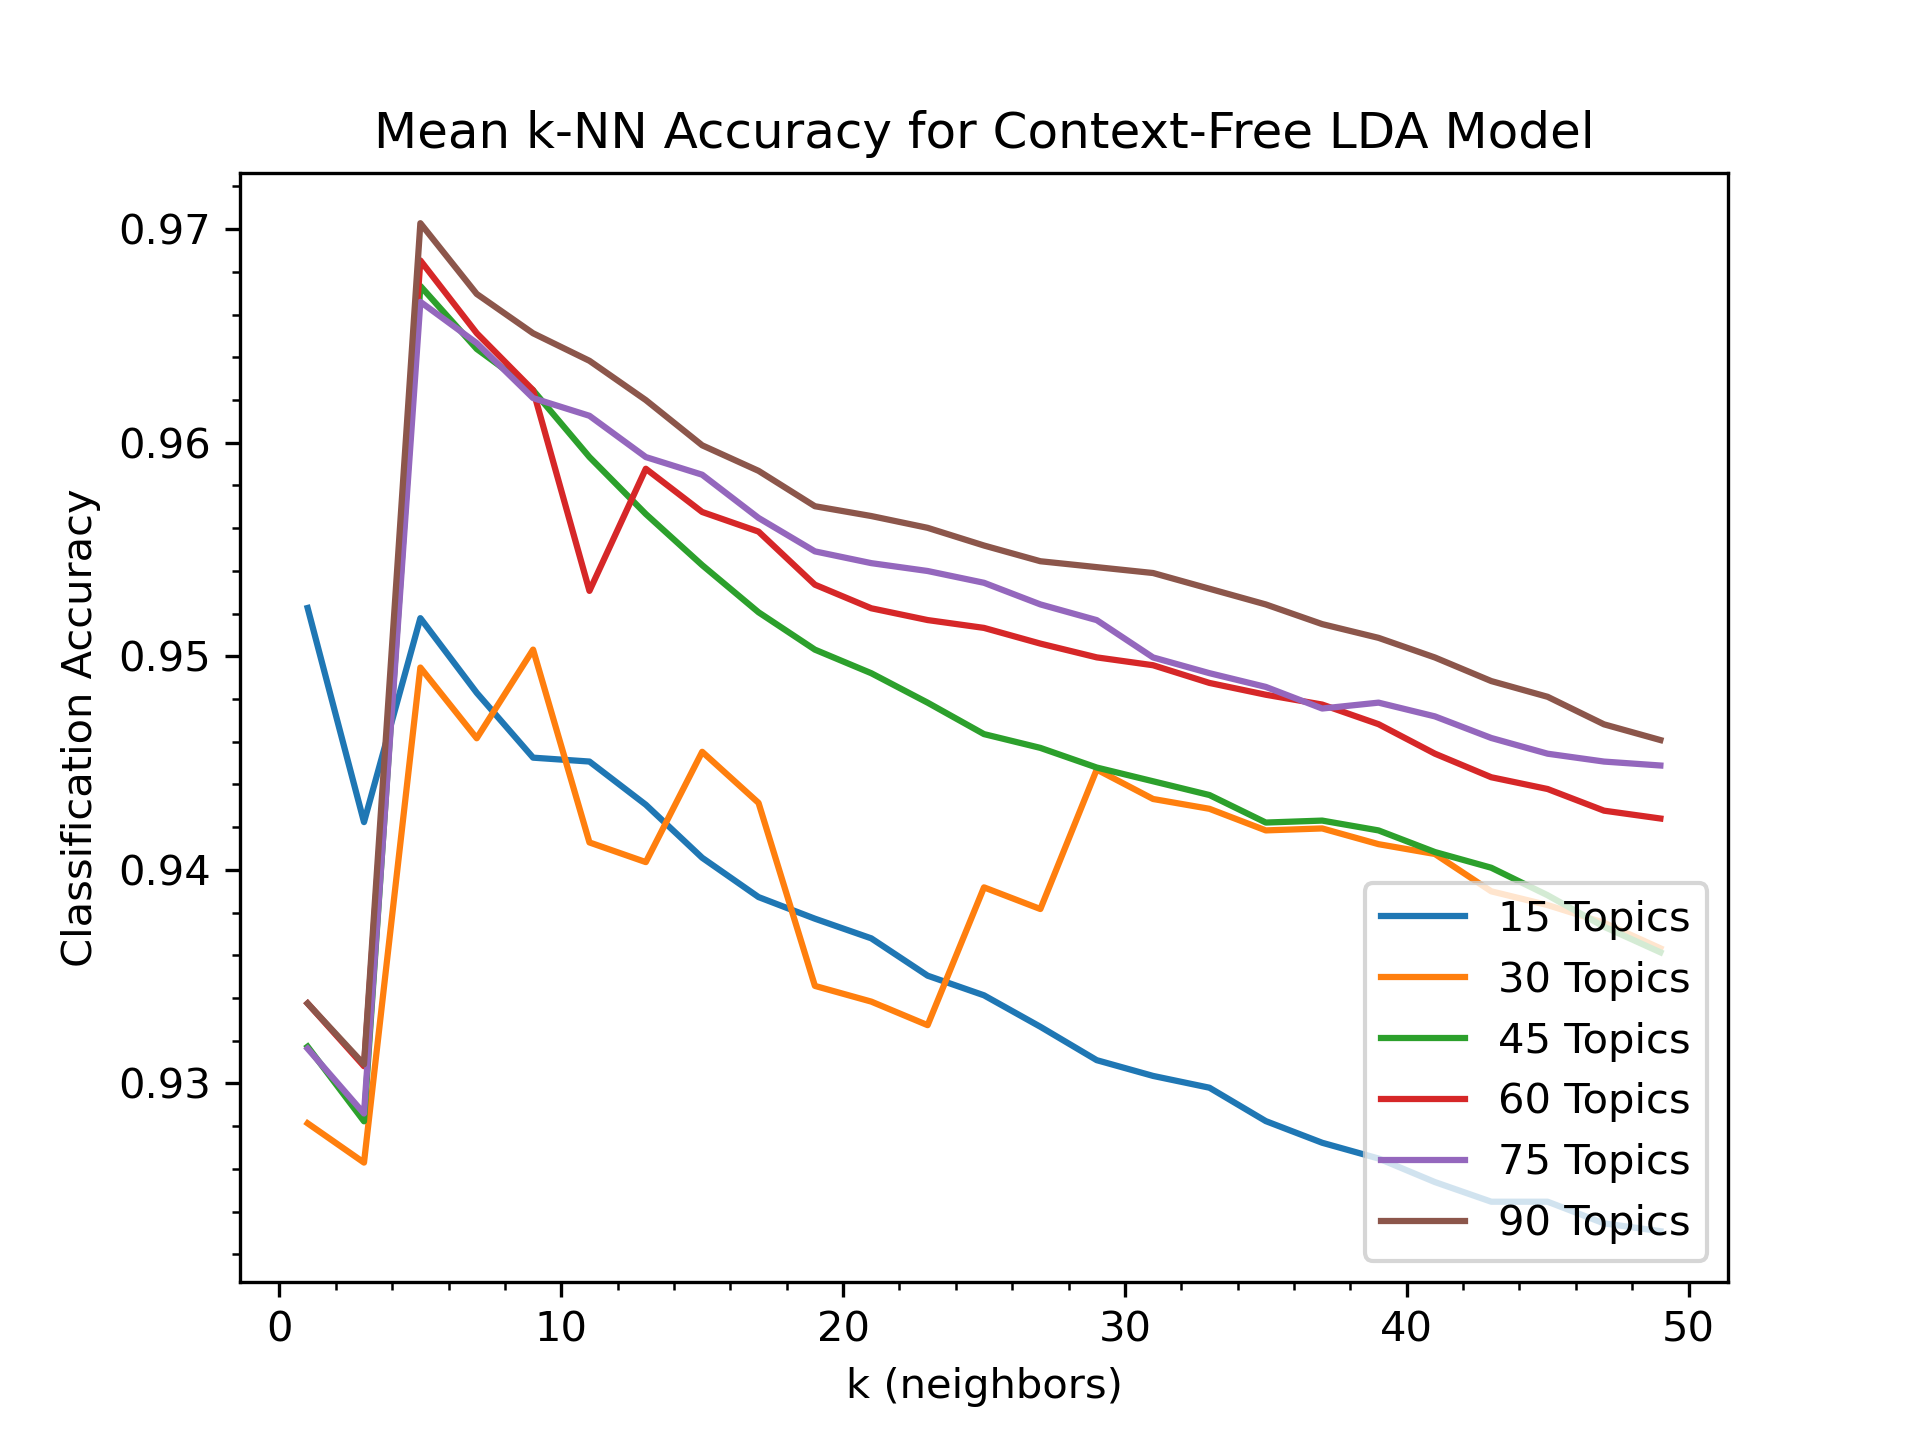
\includegraphics[width=0.75\textwidth]{img/msoft_big/knn_lda.png}
	\caption[Context-free model k-NN accuracy vs number of topics for BIG 2015]{%
		Context-free model k-NN accuracy vs $k$ for BIG 2015.
		For visual clarity, not all numbers of topics are shown and error bars are
		not included.
	}%
	\label{fig:msoft_big_knn_topics}
\end{figure}
\begin{figure}[p]
	\centering
	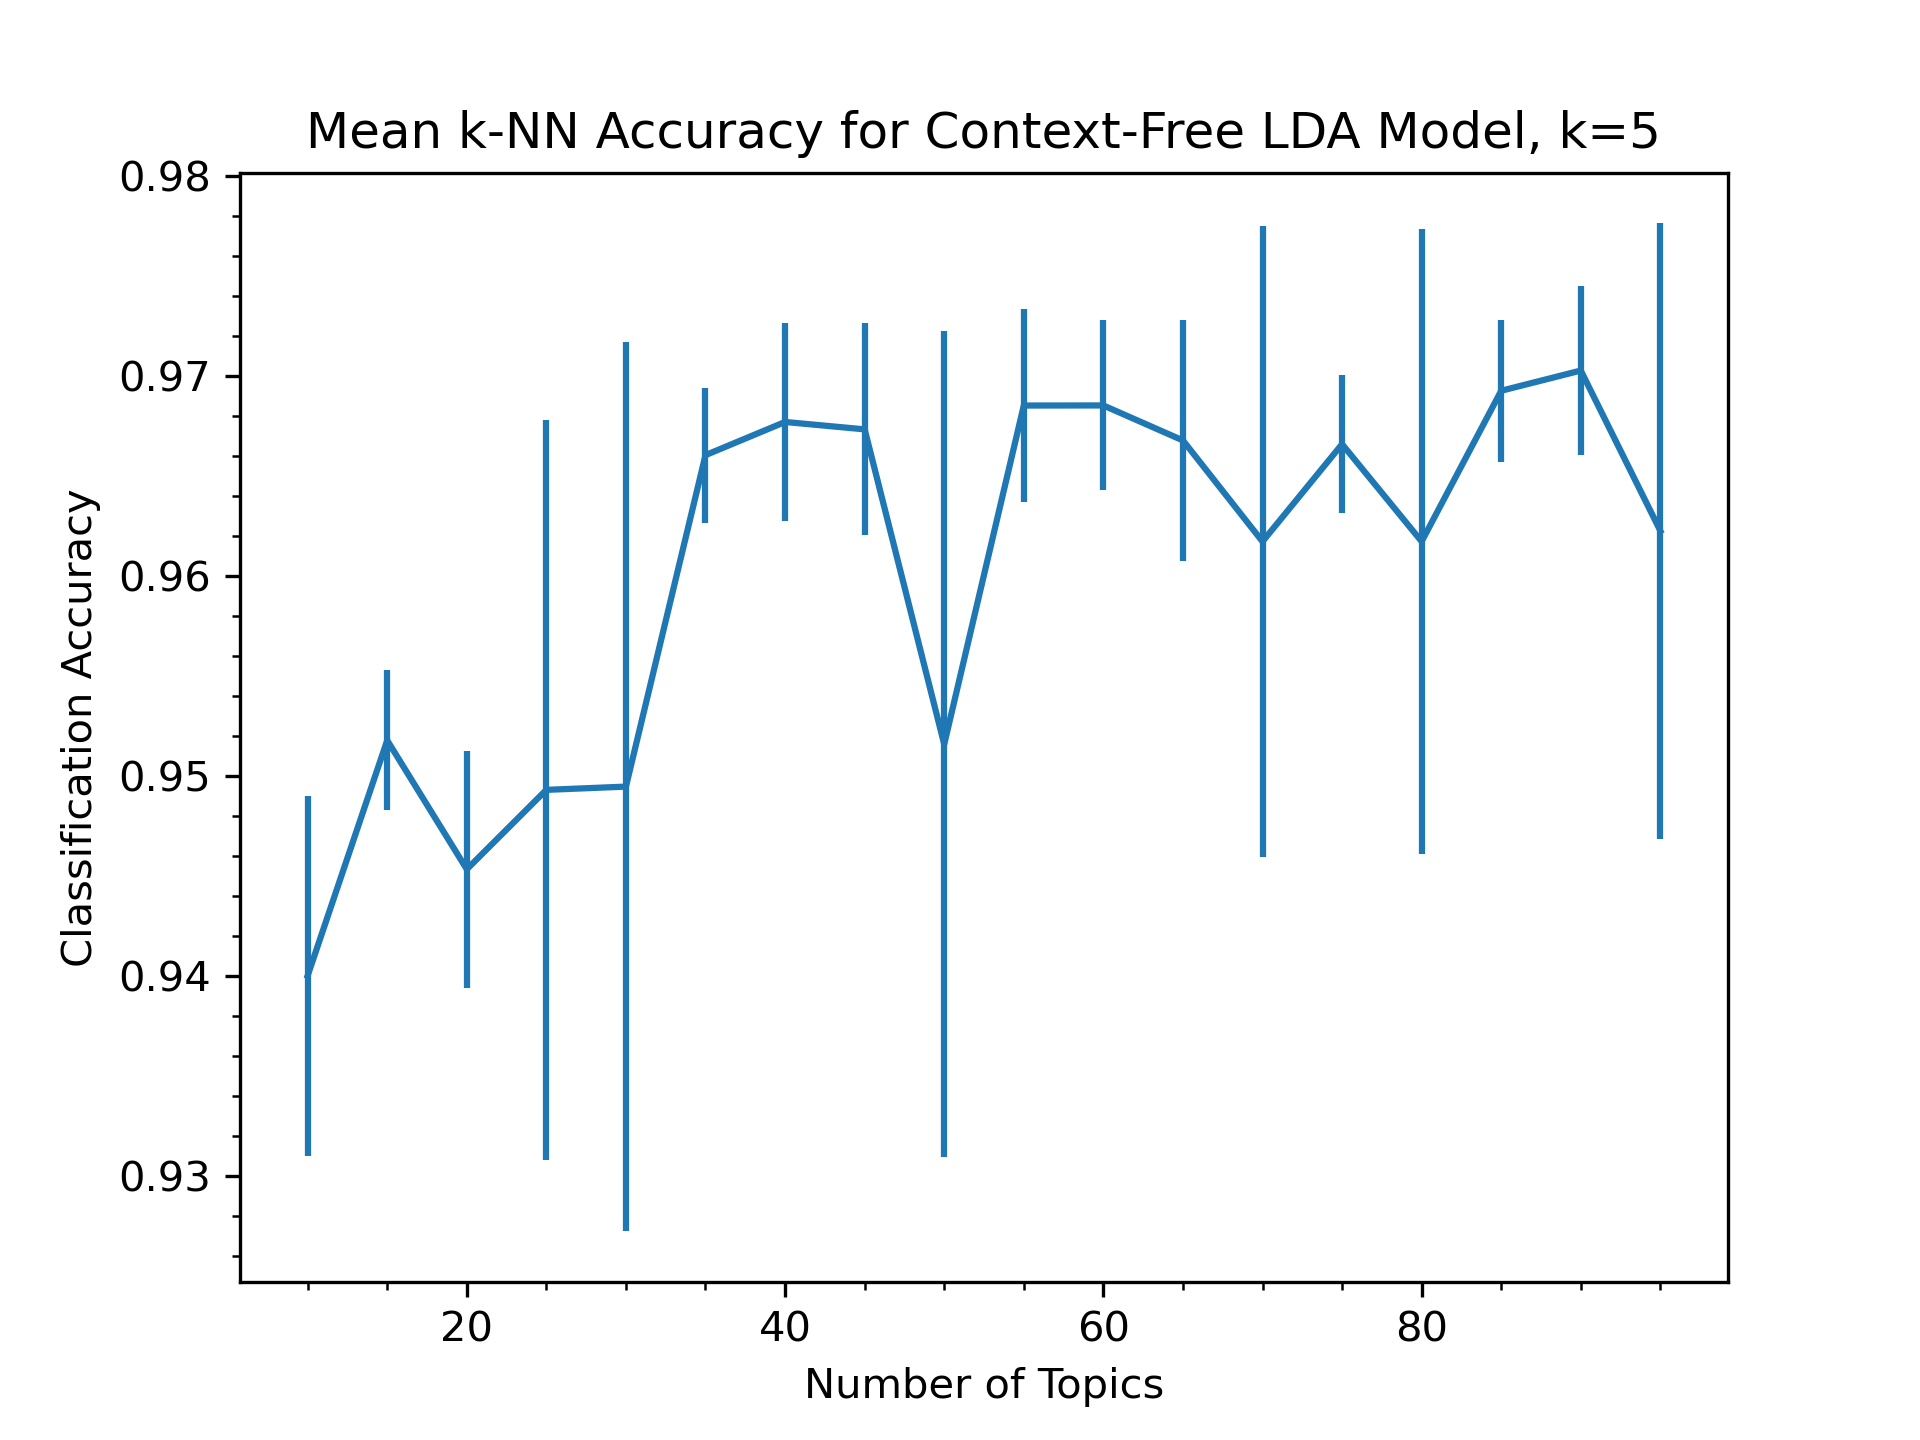
\includegraphics[width=0.75\textwidth]{img/msoft_big/knn_lda_k_05.png}
	\caption[Context-free model k-NN accuracy vs number of topics for BIG 2015]{%
		Context-free model k-NN accuracy vs number of topics for BIG 2015 fixed at
		$k=5$.
		For visual clarity, the 5 topic model is excluded.
	}%
	\label{fig:msoft_big_knn_k5}
\end{figure}

\section{Context Bit Model}%
\label{sec:res_context_bit}

\par The context bit model (trained on Das Malwerk) for various numbers of LDA
topics is shown in \figref{fig:context_bit_topic}.
As with the context-free model for Das Malwerk, the context bit model exhibits
a trend where the maximum classification performance occurs at $k=1$.
To better compare the performance of all of the LDA models (except for 5
topics), we plotted their performance with $k$ fixed at 1, shown in
\figref{fig:context_bit_k1}.
The maximal performance occurs with 45 LDA topics at $k=1$, with a
classification accuracy of 94.92\%.

% Context bit results
\begin{figure}[p]
	\centering
	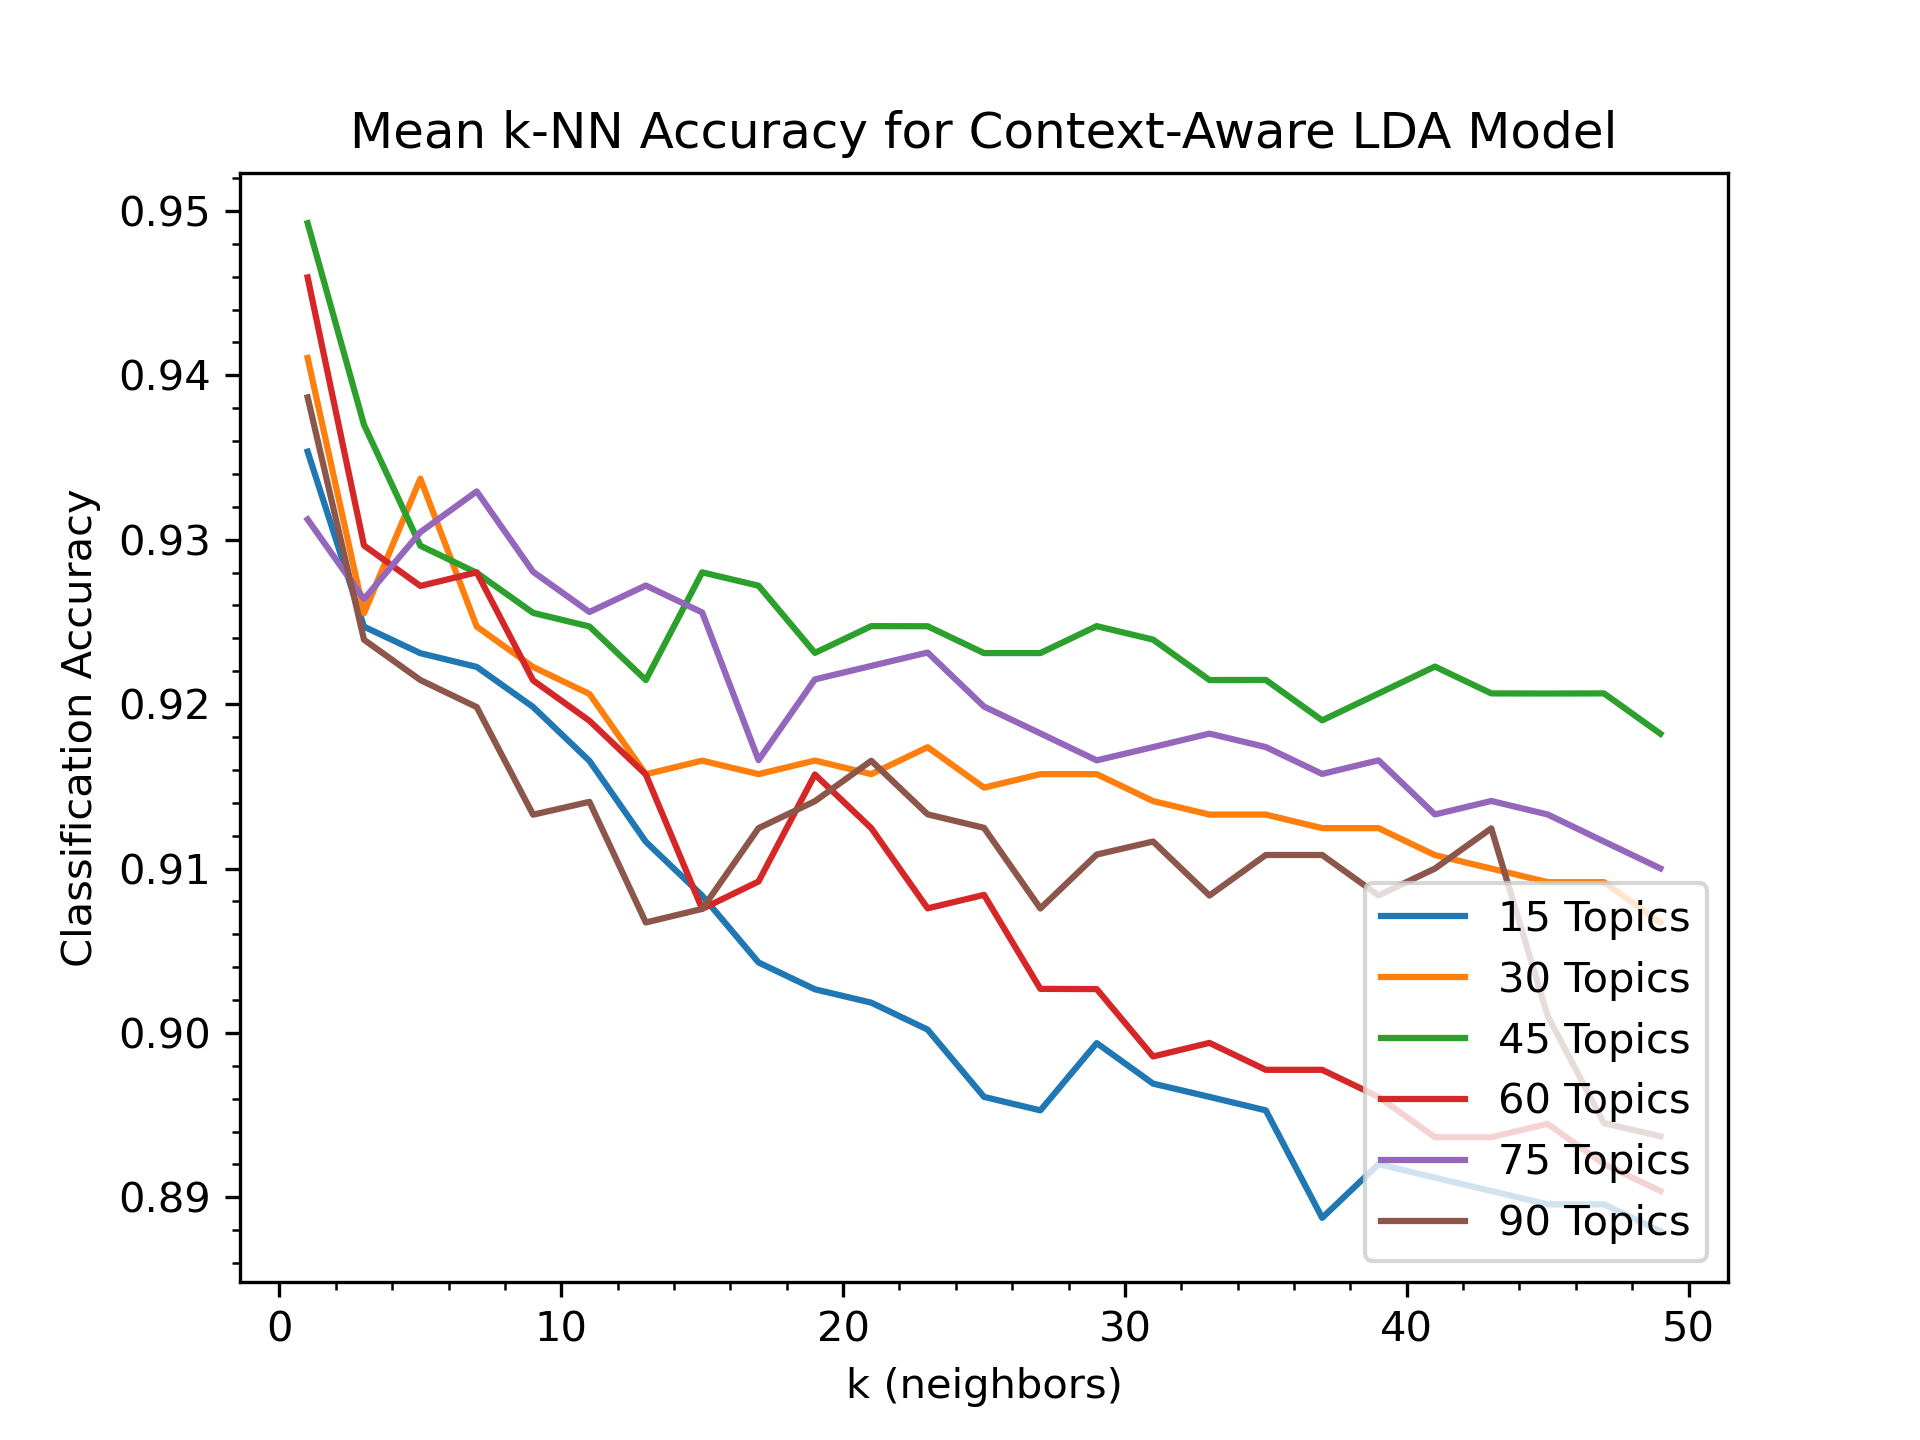
\includegraphics[width=0.75\textwidth]{img/win32/knn_lda_context.png}
	\caption[Context bit model k-NN accuracy vs $k$]{%
		Context model bit k-NN accuracy vs $k$.
		For visual clarity, not all numbers of topics are shown and error bars are
		not included.
	}%
	\label{fig:context_bit_topic}
\end{figure}
\begin{figure}[p]
	\centering
	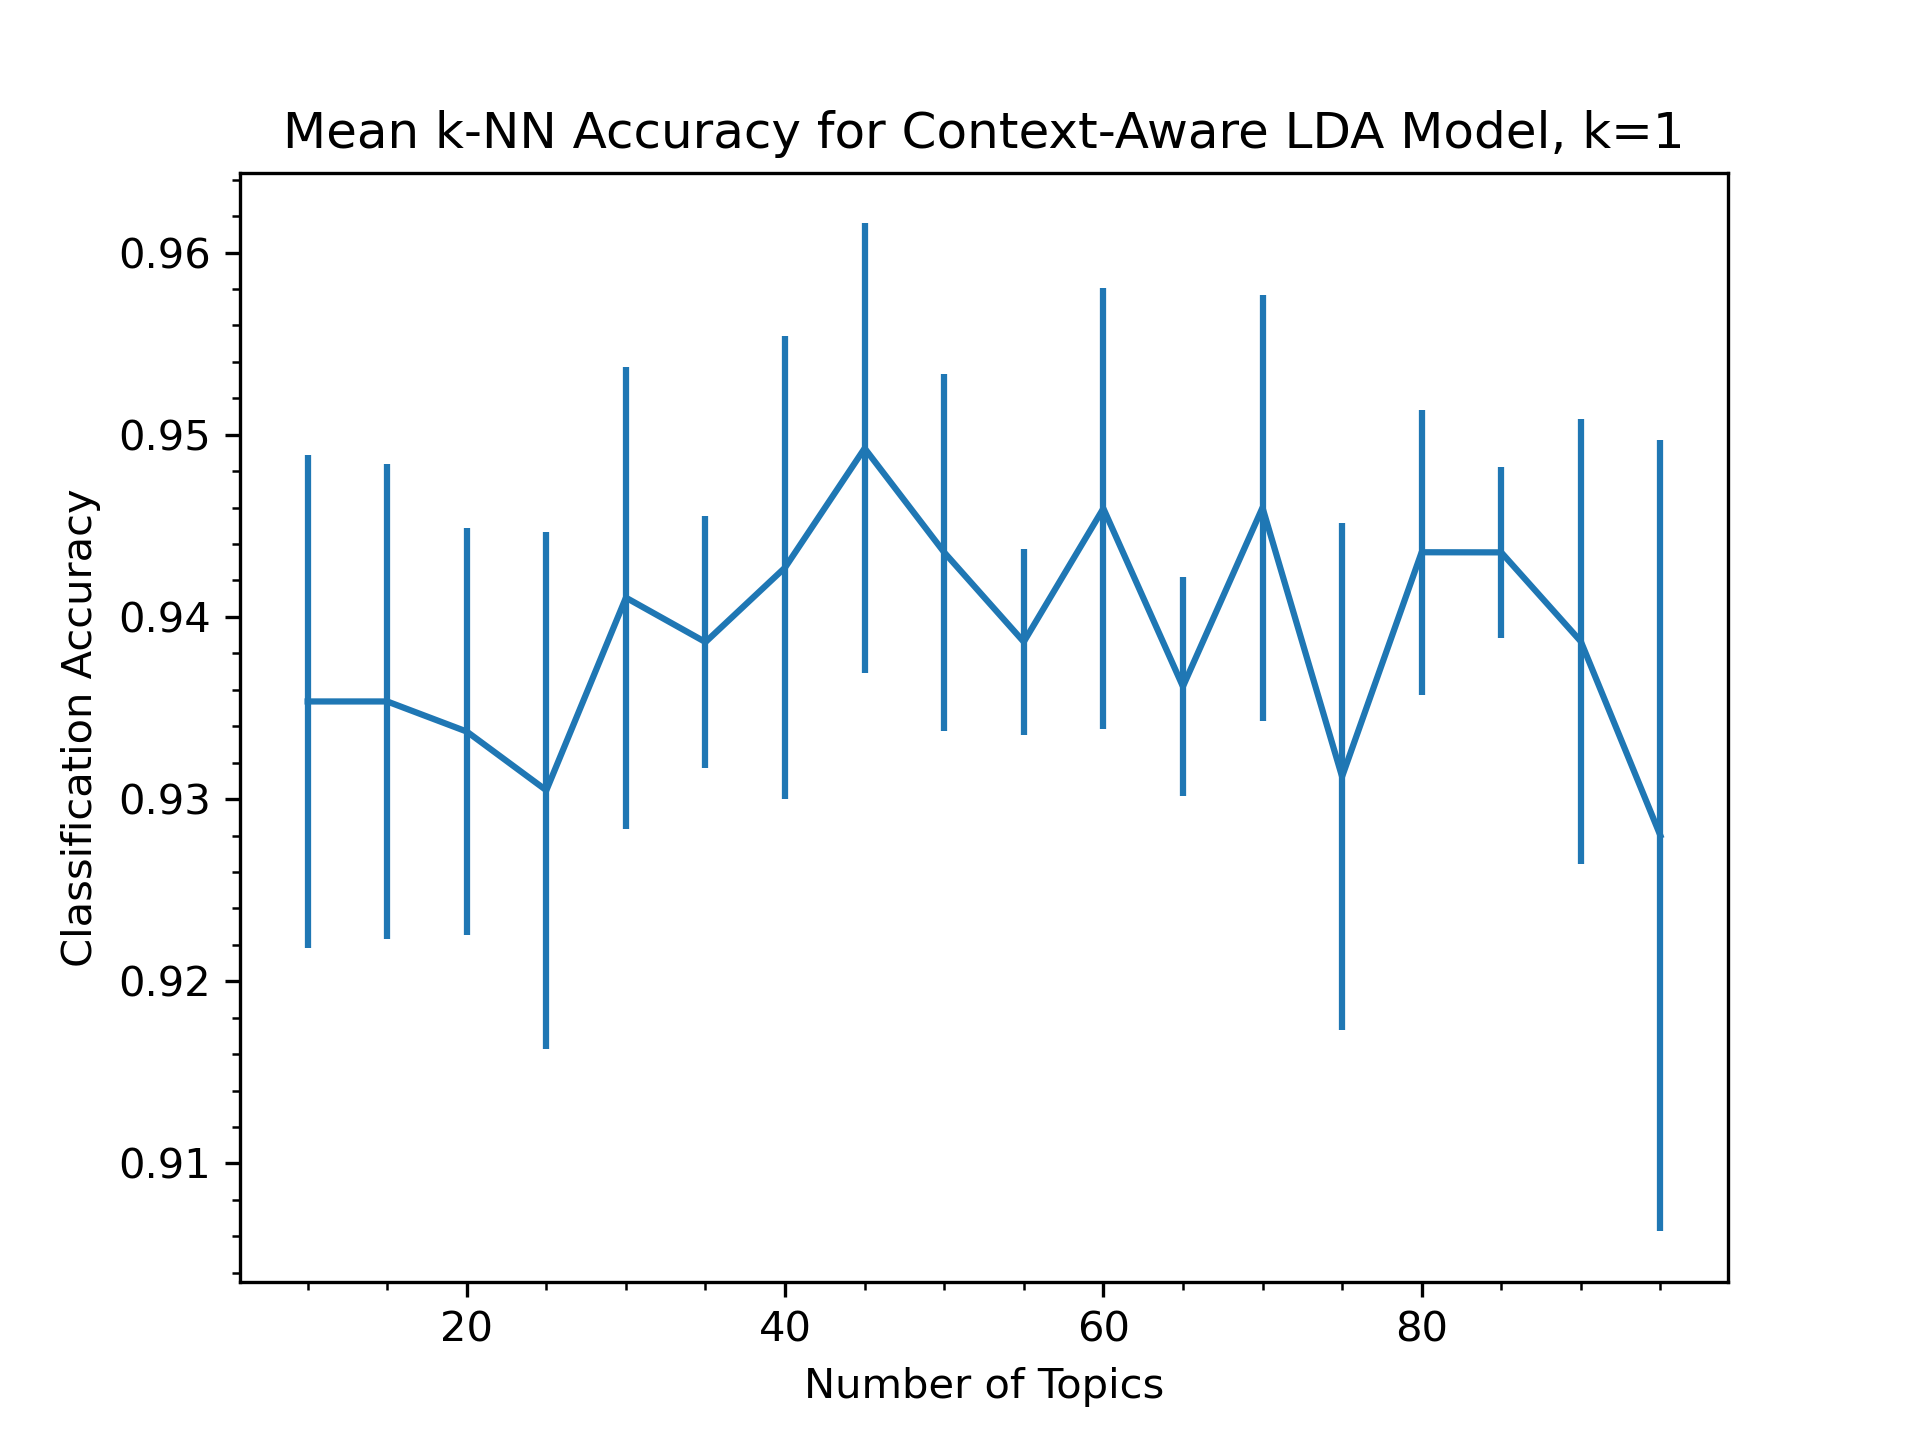
\includegraphics[width=0.75\textwidth]{img/win32/knn_lda_context_k_01.png}
	\caption[Context bit model k-NN accuracy vs number of topics]{%
		Context bit model k-NN accuracy vs number of topics fixed at $k=1$.
		For visual clarity, the 5 topic model is excluded.
	}%
	\label{fig:context_bit_k1}
\end{figure}

\section{Expected Behavior Model}%
\label{sec:res_expected_behavior}

\par The expected behavior context model (trained on BIG 2015) for various
numbers of LDA topics is shown in \figref{fig:expected_behavior_topic}.
As with the context-free model for BIG 2015, all of the models have their best
accuracies at $k=5$.
A plot showing all of the LDA models with $k$ fixed at 5 is shown in
\figref{fig:expected_behavior_k5}.
The best performance occurs with 75 topics at $k=5$, with a classification
accuracy of 97.72\%.

% Expected behavior results
\begin{figure}[p]
	\centering
	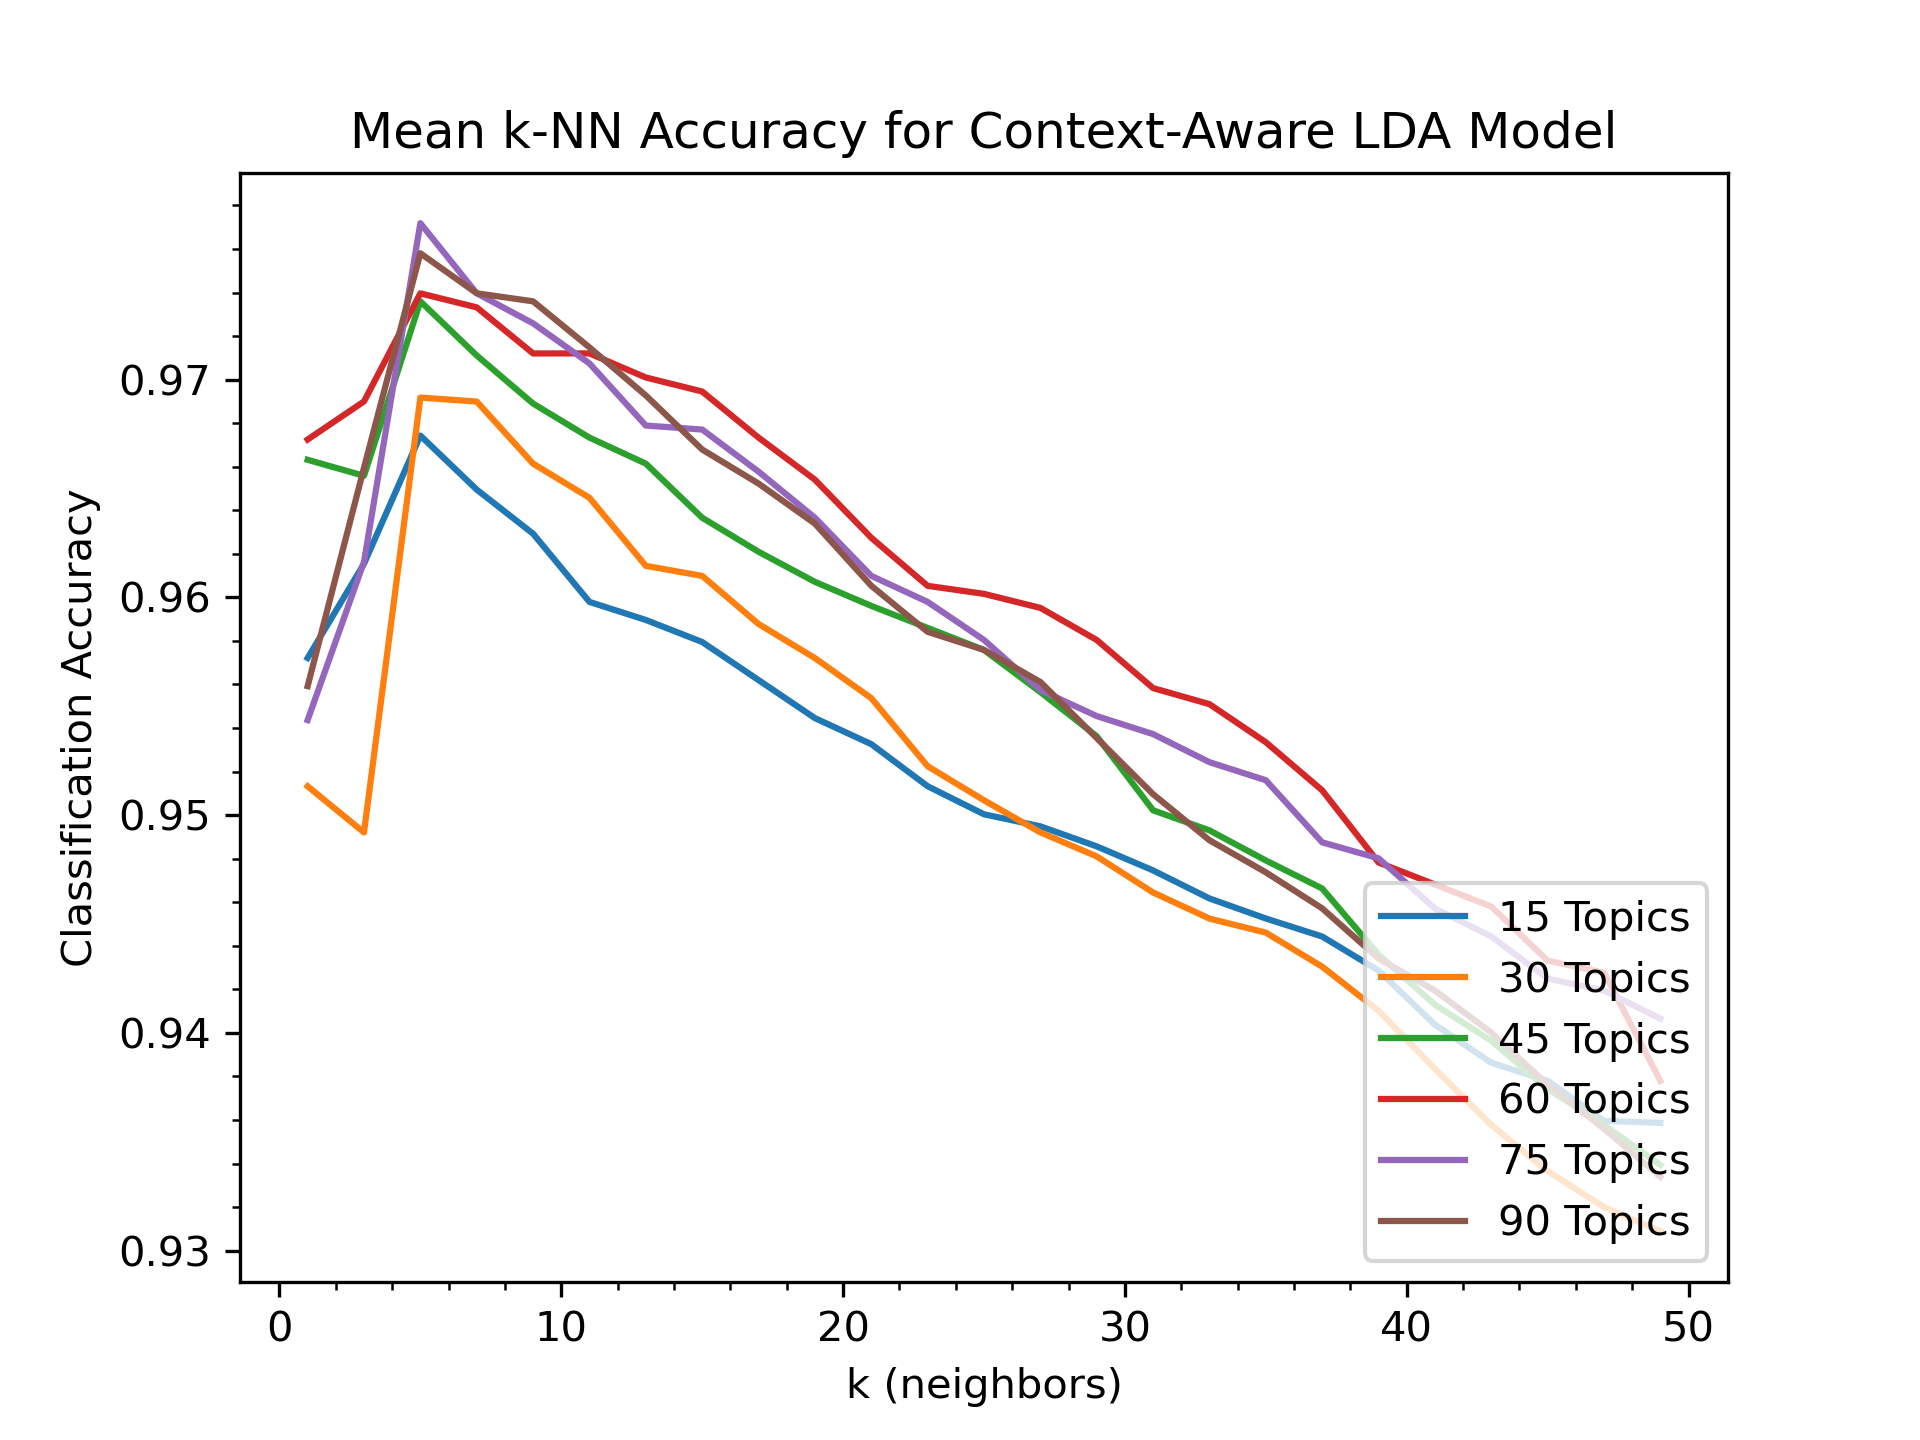
\includegraphics[width=0.75\textwidth]{img/msoft_big/knn_lda_context.png}
	\caption[Expected behavior model k-NN accuracy vs $k$]{%
		Expected behavior model k-NN accuracy vs $k$.
		For visual clarity, not all numbers of topics are shown and error bars are
		not included.
	}%
	\label{fig:expected_behavior_topic}
\end{figure}
\begin{figure}[p]
	\centering
	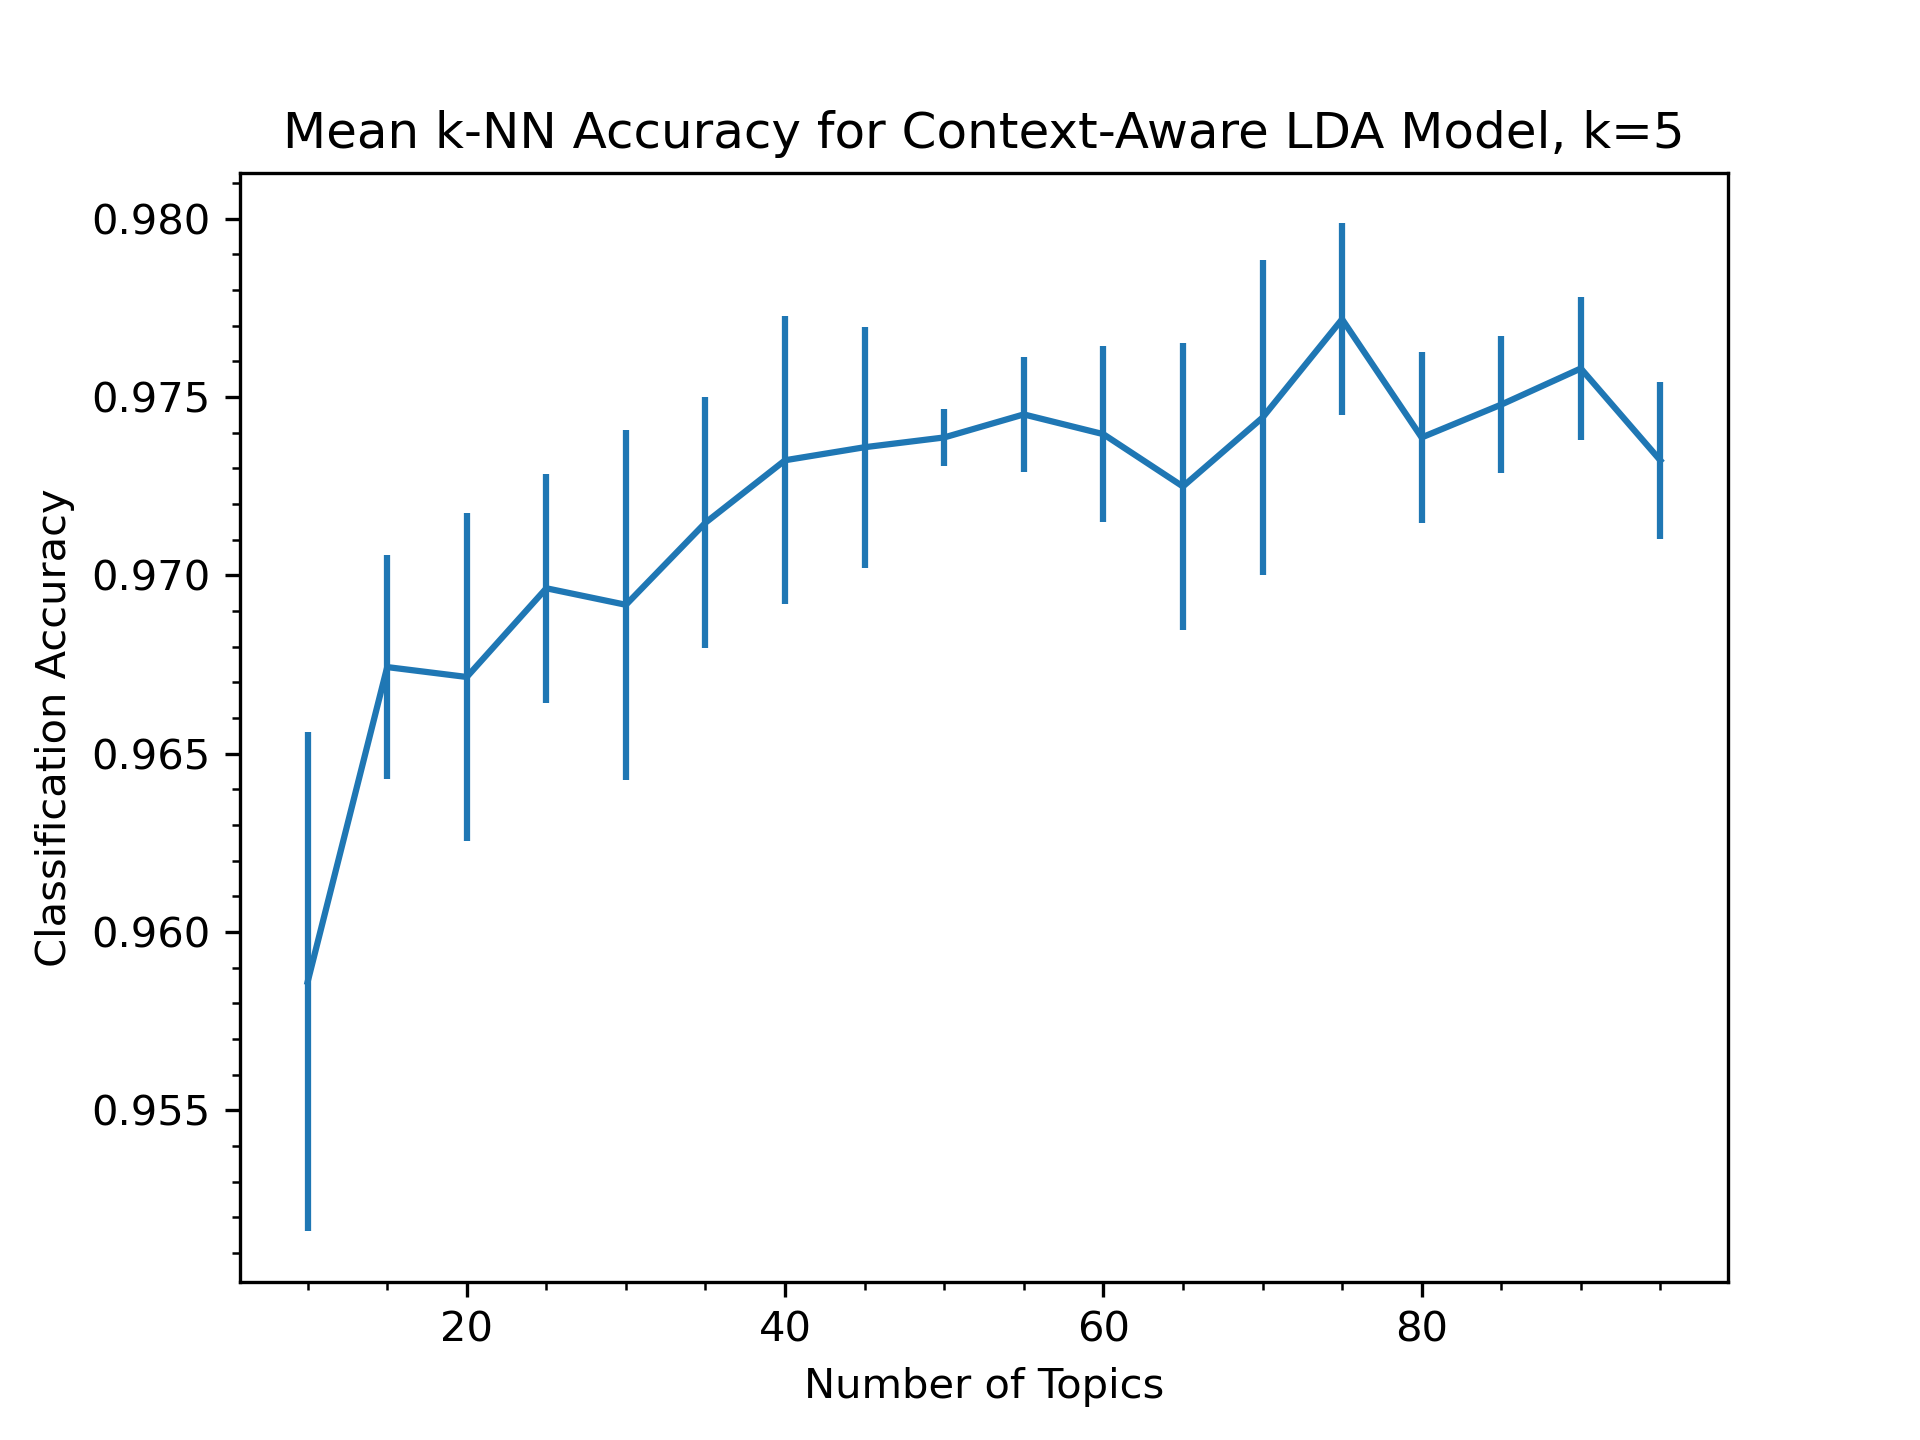
\includegraphics[width=0.75\textwidth]{%
		img/msoft_big/knn_lda_context_k_05.png%
	}
	\caption[Expected behavior model k-NN accuracy vs number of topics]{%
		Expected behavior model k-NN accuracy vs number of topics fixed at $k=5$.
		For visual clarity, the 5 topic model is excluded.
	}%
	\label{fig:expected_behavior_k5}
\end{figure}

\section{Discussion}%
\label{sec:res_discussion}

\par The context-free model shows good performance on both the Das Malwerk and
the BIG 2015 datasets, showing performance on par with other works utilizing
LDA for malware detection.
Therefore, we have shown that LDA features are useful for distinguishing the
different classes from each other.
The error bars are large and overlapping for many of the LDA models due to the
randomness involved in fitting the LDA models.
While the performance generally stayed above 90\%, such large error bars make
it difficult to be confident that the best parameters we found are actually the
best and not just a fluke.
Regardless, the performance is good enough to justify the use of LDA features
for the context-aware models.

\par One thing that LDA lacks in this application is transparency for
explanations.
When LDA is used for actual natural language documents, the topics can be
interpreted intuitively.
For example, if a topic has prominent words such as ``resistor'',
``capacitor'', and ``voltage'', a human viewer could interpret this category to
be ``electronics''.
However, when the topics are made up of opcodes, it is difficult to intuitively
understand what exactly each category means.
Due to this lack of understanding of the topics, it can be challenging to
understand explanations for the given decisions.
Furthermore, the LDA and BoW models are irreversible operations, so the
explanations cannot easily propagate past those features back to the source
code.

\par An interesting pattern was that the Das Malwerk dataset always had the
best classification accuracy with $k=1$, while the BIG 2015 dataset always
had its best classification accuracy with $k=5$.
This trend was present in virtually all numbers of topics for both the
context-free and context-aware models.

\par The context bit model shows good performance for the task we designed.
The performance was a bit lower than the context-free system, which was
expected because this implementation is essentially equivalent to injecting
noise into the system.
The issue is that the task was oversimplified.
For this model, the physical context is reduced to a single binary value.
In reality, the physical context will be a much more complicated issue.
The takeaway from this model is that the focus should be on the portion which
we black-boxed for this study, which is the model which interprets the physical
data into a context.
Additionally, the physical context alone does not form a complete context, and
it requires inclusion of other aspects of context.

\par The expected behavior context model performs its intended task very well.
One area which might impact the performance is the way the labels are
generated.
If the class identifier is changed, the program is marked as a context
violation, regardless of what class it was switched to.
However, if two classes are similar to each other, it is possible that their
LDA topic distributions are expected to be similar.
This issue was considered, but the performance is high enough to demonstrate
the desired concept.

\newpage

\end{document}
